\documentclass{beamer}

\usepackage[T1]{fontenc}
\usepackage[utf8]{inputenc}
\usepackage{graphicx}
\usepackage{tikz}
\usepackage{epigraph}
\usepackage{txfonts}
\usepackage{hyperref}
\usepackage[outputdir=./out]{minted}

\usetikzlibrary{fadings}
\usetikzlibrary{shadows}
\usetheme[circularprogress=true]{BayooTec}
\usemintedstyle{one-dark}

\definecolor{sourcebg}{HTML}{131a24}

\newminted{ruby}{
  fontsize=\scriptsize,
  numbersep=8pt,
  gobble=4,
  bgcolor=sourcebg,
}

\title{Code is Music}
\subtitle{Eine Einführung ins Live-Coding}
\author{Martin Gondermann}
\date{\today}

\setlength{\epigraphwidth}{0.5\textwidth}

\newenvironment{colortheme}[1]{
  \input beamercolortheme#1.sty
}{}

\begin{document}

% Startseite
\begin{frame}[plain]
  \titlepage%
\end{frame}
\addtocounter{framenumber}{-1}

\begin{frame}
  \frametitle{Über mich}
  \begin{columns}
    \column{0.2\textwidth}
    \column{0.6\textwidth}
    \centering
    \begin{tikzpicture}
      \usebeamercolor{palette primary}\fill[fg, circular drop shadow={shadow scale=1.02,shadow xshift=0.6ex, shadow yshift=-0.6ex}] (0, 0) circle [radius=2cm];
      \clip (0, 0) circle (1.9cm);
      \node[anchor=center] at (0, 0) {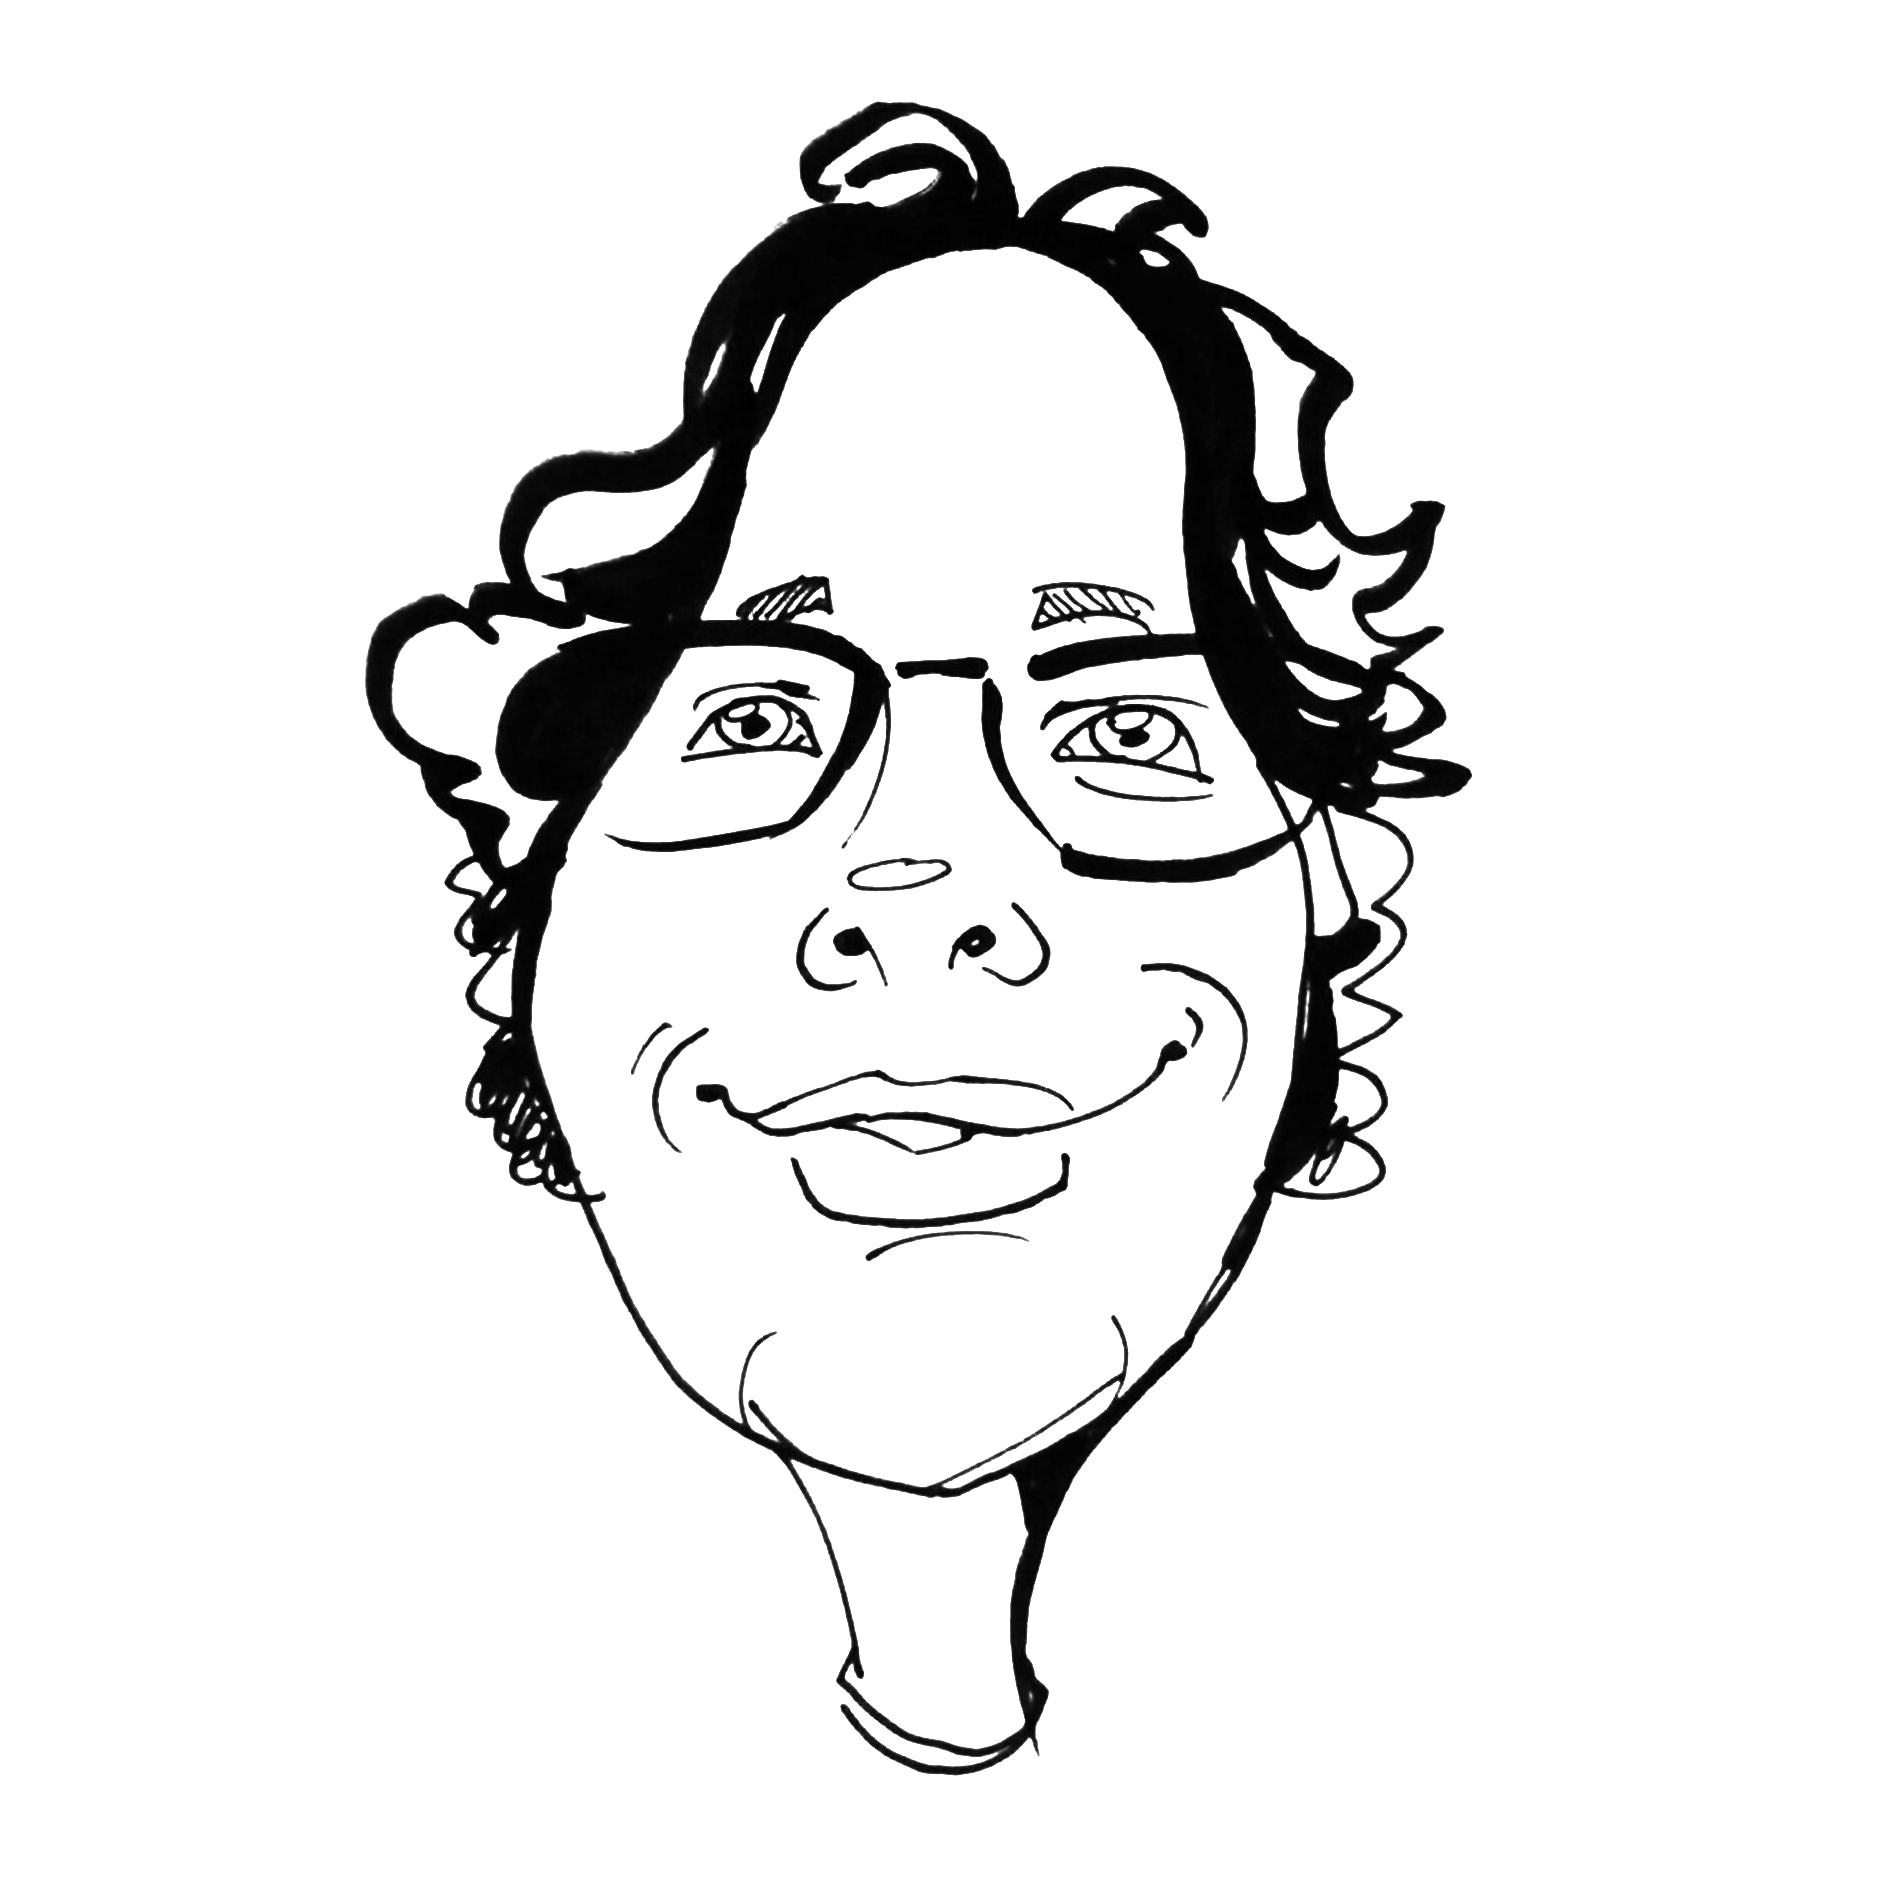
\includegraphics[width=3.9cm]{images/karikatur.png}};
    \end{tikzpicture}

    \vspace{0.5ex}
    \usebeamercolor[fg]{palette primary}\textbf{\textit{Martin Gondermann}}

    \usebeamercolor[fg]{palette secondary}\textit{Senior Software Engineer, Bayootec}
    \column{0.2\textwidth}
  \end{columns}
\end{frame}
\addtocounter{framenumber}{-1}

\begin{colortheme}{Lambdaphonic}
  \begin{frame}
    \frametitle{Über mich}
    \framesubtitle{The dark side}
    \usebeamercolor[fg]{palette primary}
    \begin{columns}
      \column{0.2\textwidth}

      \column{0.6\textwidth}
      \centering
      \begin{tikzpicture}
        \usebeamercolor{palette primary}\fill[fg, circular drop shadow={shadow scale=1.02,shadow xshift=0.6ex, shadow yshift=-0.6ex}] (0, 0) circle [radius=2cm];
        \clip (0, 0) circle (1.9cm);
        \usebeamercolor{background canvas}\fill[bg, circular drop shadow={shadow scale=1.02,shadow xshift=0.6ex, shadow yshift=-0.6ex}] (0, 0) circle [radius=1.9cm];
        \node[anchor=center] at (0, 0) {
\includegraphics[width=3cm]{images/lambdaphonic.png}};
      \end{tikzpicture}

      \vspace{0.5ex}
      \textit{$\lambda$phonic}

      \usebeamercolor[fg]{palette secondary}
      \textit{Live coder}

      \usebeamercolor[fg]{palette tertiary}
      \small\url{https://lambdaphonic.de}

      \column{0.2\textwidth}
    \end{columns}
  \end{frame}
\end{colortheme}

\section{Was ist Live Coding?}
\subsection{Definition}
\begin{frame}
  \frametitle{Was ist Live Coding?}
  \framesubtitle{TOPLAP}
  \small
  \begin{itemize}
    \item Give us access to the performer's mind, to the whole human instrument.
    \item Obscurantism is dangerous. Show us your screens.
    \item Programs are instruments that can change themselves
    \item The program is to be transcended --- Artificial language is the way.
    \item Code should be seen as well as heard, underlying algorithms viewed as well as their visual outcome.
    \item Live coding is not about tools. Algorithms are thoughts. Chainsaws are tools. That's why algorithms are sometimes harder to notice than chainsaws.
  \end{itemize}
\end{frame}

\begin{frame}
  \frametitle{Was ist Live Coding?}
  \framesubtitle{Definition}
  The Live Coder creates and manipulates source code live in front of an audience.

  \vspace{1ex}
  He combines code, music and visuals into a synaestetic performance.
\end{frame}

\begin{frame}
  \frametitle{Was ist Live Coding?}
  \framesubtitle{Definition}
  \renewcommand{\epigraphflush}{center}
  \epigraph{
    \usebeamercolor{palette primary}
    \textbf{\textcolor{fg}{Live}} coding music, \\
    \textbf{\textcolor{fg}{Electronic}} notes dance and flow, \\
    \textbf{\textcolor{fg}{Algorithms}} sing.
  }{\usebeamercolor{palette secondary}\textcolor{fg}{\textit{Haiku by Chat GPT}}}
\end{frame}

\section{Geschichte}
\begin{frame}
  \frametitle{Geschichte}
\end{frame}

\section{Live Coding Systeme}
\begin{frame}
  \frametitle{Live Coding Systeme}
  \framesubtitle{Eine Auswahl}
  \begin{columns}
    \column{0.5\textwidth}
    \begin{itemize}
      \item Supercollider
        \begin{itemize}
          \item Die ``Mutter'' der meisten Live Coding Systeme
        \end{itemize}
      \item Gibber (Web / JavaScript)
      \item Orca (Visual~``Programming'')
      \item Tidal Cycles (Haskell~based)
      \item Overtone (Clojure)
    \end{itemize}

    \column{0.5\textwidth}
    \begin{itemize}
      \item GLICOL (Rust)
      \item FoxDot (Python)
      \item Extempore (Scheme~based)
      \item Sonic Pi (Ruby)
    \end{itemize}
  \end{columns}
\end{frame}

\section{Sonic Pi}
\subsection{Basics}
\begin{frame}{Sonic Pi}{Basics}
  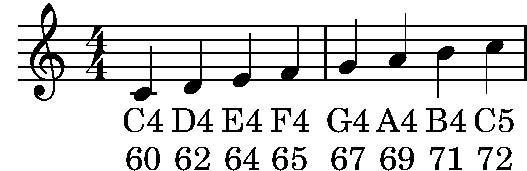
\includegraphics{images/scale.pdf}
\end{frame}

\begin{frame}[fragile]{Sonic Pi}{Basics}
  \begin{rubycode}

    # spielt die Note C4 mit dem aktuell ausgewählten Instrument
    play :C4
    play 60 # das Selbe, nur in MIDI notation

    # spielt mehrere Noten (Akkord) gleichzeitig
    play :C4
    play :E4
    play :G4

    # spielt die Noten nacheinander ab (1/4 Noten)
    play :C4
    sleep 0.25
    play :E4
    sleep 0.25
    play :G4
    sleep 0.25

  \end{rubycode}
\end{frame}

\subsection{Zufall/Randomisierung}
\begin{frame}[fragile]{Sonic Pi}{Zufall/Randomisierung}
  \begin{rubycode}

    # Zufallswerte
    rand()          # Zufallszahl zwischen 0.0 und 1.0
    rand(0.5)       # Zufallszahl zwischen 0.0 und 0.5
    rand(0.1..0.8)  # Zufallszahl zwischen 0.1 and 0.8
    rand_i(5)       # Zufällige Ganzzahl (eine von 0, 1, 2, 3, 4)
    rdist(1, 0)     # Zufallszahl zwischen -1.0 und 1.0
    rrand(6, 10.5)  # Zufallszahl zwischen 6.0 und 10.5 inklusive
    rrand_i(6, 10)  # Zufällige Ganzzahl zwischen 6 and 10 inklusive
    dice            # würfelt (6-seitiger Würfel) (1-6 inklusive)
    dice(3)         # würfelt (3-seitiger Würfel)
    one_in(3)       # true mit Wahrscheinlichkeit von 1/3

    # Listen-Operatoren
    [1, 2, 3].pick(2)   # Wählt 2 zufällige Einträge aus der Liste
    [1, 2, 3].shuffle   # Liste mischen
    [60, 64, 67].choose # Zufälligen Eintrag auswählen

  \end{rubycode}
\end{frame}

\subsubsection{Beispiele}
\begin{frame}[fragile]{Sonic Pi}{Zufall/Randomisierung --- Beispiele}
  \begin{rubycode}

    # zufällige Note des A-moll Akkords spielen
    play chord(:A4, :minor).choose

    # Sample mit einer Wahrscheinlichkeit von 50% (1/2) abspielen
    sample :drum_cymbal_pedal if one_in(2)

    # spielt das Sample mit einer zufälligen Lautstärke
    sample :drum_cymbal_pedal, amp: rand(0.4..0.8)

  \end{rubycode}
\end{frame}

\section{Konzepte}
\subsection{Temporal Recursion}
\begin{frame}
  \frametitle{Konzepte}
  \framesubtitle{Temporal recursion}
\end{frame}

\subsection{Live Loop}
\begin{frame}
  \frametitle{Konzepte}
  \framesubtitle{Live Loop}
\end{frame}


\subsection{Euklidische Patterns}
\begin{frame}
  \frametitle{Konzepte}
  \framesubtitle{Euklidische Patterns}
\end{frame}

\end{document}
